\chapter{Componentes que forman el vehículo}

Como brazo ejecutor del sistema se ha decidido integrar una serie de componentes con los cuales se pueda llevar a cabo la conducción, comunicación, y traducción de la información en movimientos. A continuación se va a proceder a explicar en cada uno de los apartados el porqué se han elegido dichos componentes.

\section{\emph{Arduino} UNO R3 ATMEGA328}

Ejerce de plataforma computacional con la que se controlan todos los elementos de prototipado que, en su conjunto, forman el vehículo. Lo bueno del uso de esta placa es que nos permite integrar el uso de sensores, motores y módulos de comunicación. Lo cual es perfecto ya que nos permite diseñar un vehículo en función de nuestras necesidades.

\section{Controlador \emph{Sparkfun} Ardumoto y chasis}

El laboratorio \emph{ARCO} concedío para este proyecto un chasis en el cual vienen instalados cuatro motores de corriente contínua de 9V conectados a un  controlador Ardumoto de la marca \emph{Sparkfun}. Este artilugio permite obtener resultados muy rápido ya que mediante el uso de estos cuatro pines digitales se puede emular el movimiento de un coche:

\begin{itemize}
\item DIRA 12 y DIRB 13: Con el valor de salida 0 las ruedas giran en sentido de las agujas del reloj y con la salida a 1 en sentido antihorario.
\item PMWA 3 y PMWA 11: Permiten configurar la velocidad de rotación de los motores. El rango de velocidad se encuentra entre 0 (parado) y 255 (máxima velocidad). 
\end{itemize}

\begin{figure}[hbtp]
 \centering
   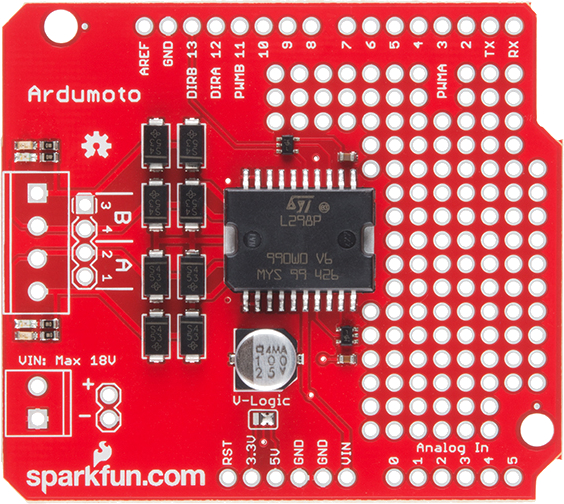
\includegraphics[width=0.6\textwidth]{./figures/ardumoto.jpeg}
 \caption{Ardumoto}
 \label{fig:Ardumoto}
\end{figure}

\section{Módulos \emph{Xbee} de la marca \emph{Digi}}

Mediante el uso de estos módulos de comunicación por radio se puede establecer una comunicación por puerto serie entre \emph{Arduino} y la placa \emph{Zedboard}. Igual que con el controlador ardumoto, la aplicación de este módulo nos proporciona rápidos resultados. Esto es debido a que gracias al manejo de un adaptador microusb de la marca \emph{Sparkfun} y el software \emph{XCTU} de la marca \emph{Digi} se realiza una configuración entre ambos módulos que permite establecer la comunicación entre ambos y simplifica la interacción con la placa \emph{Arduino} al uso de 2 pines, obviando los pines de alimentación:

\begin{itemize}
\item DIN y DOUT mediante los cuales se establece la comunicación de entrada y salida por el puerto serie. 
\end{itemize}

\begin{figure}[htbp]
 \centering
  \subfloat[Módulo \emph{Xbee}]{
    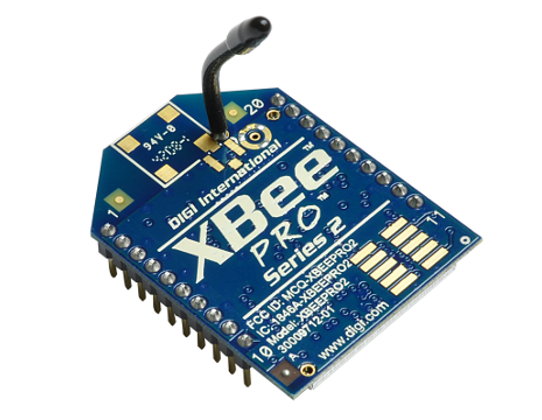
\includegraphics[width=0.4\textwidth]{./figures/Xbee.png}}
  \subfloat[Adaptador microusb]{
    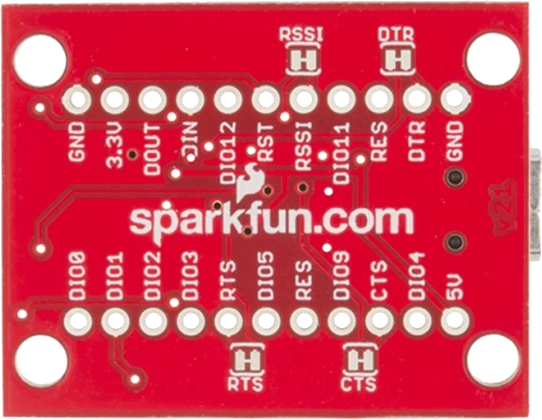
\includegraphics[width=0.4\textwidth]{./figures/XbeeSparkfun.png}}
 \caption{Módulo de comunicación del sistema}
 \label{fig:Xbee}
\end{figure}

\section{Batería recargable \emph{Odec} 9V}

Se ha decidido utilizar pilas recargables \emph{Odec} 9V de 600mAh de salida debido a que por el número de componentes que forman el vehículo, el consumo del coche es grande. En un principio se utilizaron pilas de 9V no recargables y se consumían en un día de pruebas, lo cual generaba un coste innecesario debido a que se debían comprar pilas muy frecuentemente.

\section{Osciloscopio y multímetro}

El laboratorio \emph{ARCO} posee un multímetro \emph{BEHA} 93423 con el cual se han realizado medidas de voltaje sobre el prototipado del proyecto. Este artilugio ha sido de gran utilidad ya que en un momento del proyecto se cometío un fallo de alimentación en uno de los componentes. El descuido consistío en que debido a la utilización de una base \emph{Shield} de la marca \emph{Seed}. Véase la figura \ref{fig:Shield}. Todos los pines VCC de la placa estaban configurados en 5V pero el módulo \emph{XBee} estaba utilizando el pin de 3.3V. A causa de esta negligencia el módulo \emph{XBee} dejó de funcionar ya que se alimentaba de un voltaje mayor del que soportaba. Hubo un momento en el cual no se podía ver a simple vista que ocurría en el coche. Ya que la comunicación no funcionaba. Y en un principio no se sabía que componente era el causante del mal funcionamiento. Debido a que no se producía ningún movimiento se pensó que era debído al módulo de comunicación, pero el led del adaptador microusb para \emph{XBee} funcionaba.  En primer lugar se comprobó si era por algún error en la configuración, pero tras comprobar que la configuración era correcta. Se procedío a medir los voltajes de los componentes. Fue en ese momento cuando se comprobó que el voltaje de entrada del módulo \emph{XBEE} era erróneo. El módulo \emph{XBee} fue sustituido por uno nuevo y se tomó una mayor precaución en el futuro para evitar este tipo de descuidos.

\begin{figure}[hbtp]
 \centering
   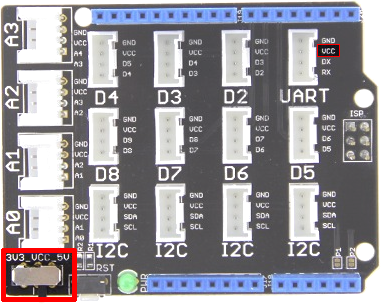
\includegraphics[width=0.7\textwidth]{./figures/shield.png}
 \caption{Placa base}
 \label{fig:Shield}
\end{figure}

\section{Placa de pruebas para Arduino}

Sobre esta tabla se establece la instalación de los sensores, leds y resistencias del coche. Esta placa de pruebas se ha utilizado como maqueta para realizar una serie de pruebas correspondientes a activar los motores, detectar el efecto Hall, encender leds y comprobar el funcionamiento del protocolo de comunicación establecido entre la placa \emph{Zedboard} y \emph{Arduino}. Además, se utiliza en la versión final del vehículo como lugar de instalación de los sensores de efecto Hall, leds y resistencias que permiten el funcionamiento de los sensores y leds. 

\section{\emph{Arduino shield}}

Imprescindible para poder utilizar los pines de \emph{Arduino} que no utiliza el controlador Ardumoto. Ya que si instalaramos la placa ardumoto sobre \emph{Arduino} inutilizaría los pines de \emph{Arduino} que no se utilizan. Véase la figura \ref{fig:ArdumotoShield}. Mientras que con el uso de la base \emph{Shield}, véase la figura \ref{fig:Shield}, se pueden utilizar todos los pines que ocupa \emph{Ardumoto}.

\begin{figure}[hbtp]
 \centering
   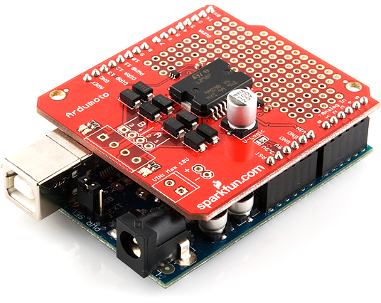
\includegraphics[width=0.5\textwidth]{./figures/ArdumotoShield.png}
 \caption{Ardumoto instalado sobre \emph{Arduino UNO}}
 \label{fig:ArdumotoShield}
\end{figure}

\section{Sensor efecto Hall A3144}

Debido a que lo motores de corriente contínua carecen de encoders\footnote{Los Encoders convierten el movimiento en una señal eléctrica que puede ser leída por algún tipo de dispositivo de control en un sistema de control de movimiento, tal como un mostrador. El encoder envía una señal de respuesta que puede ser utilizada para determinar la posición, contar, velocidad o dirección.}. Se ha decidido emular el funcionamiento de un encoder mediante el uso de un sensor de efecto Hall\footnote{Se conoce como efecto Hall a la aparición de un campo eléctrico por separación de cargas, en el interior de un conductor por el que circula una corriente en presencia de un campo magnético con componente perpendicular al movimiento de las cargas. Este campo eléctrico (campo Hall) es perpendicular al movimiento de las cargas y a la componente perpendicular del campo magnético aplicado. Lleva el nombre de su primer modelador, el físico estadounidense Edwin Herbert Hall.}. El sensor de efecto Hall permite detectar la variación producida en un campo eléctrico mediante la aproximación de un campo magnético. Si fijamos un imán de neodimio en el lateral de la rueda e instalamos un sensor pegado a esta. Cada vez que el imán pase cerca del sensor A3144, este detectará la variación del campo electrico. Si el imán se acerca al sensor devuelve el valor 0 por el pin digital, mientras que si por el contrario el imán se encuentra lejos, devuelve un 1.

\begin{figure}[hbtp]
 \centering
   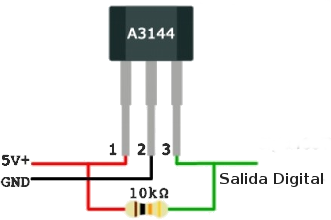
\includegraphics[width=0.5\textwidth]{./figures/SensorEH.png}
 \caption{Sensor Efecto Hall A3144}
 \label{fig:sensorEH}
\end{figure}

El uso de este sensor nos permite controlar el número de vueltas que realiza una rueda. Ya que si contamos el número de veces que el sensor devuelve un 0 por el pin digital que está conectado a \emph{Arduino}, podremos mantener un control acerca de cuanto se mueve el vehículo. Como en los casos de ejemplo la cámara cenital se coloca a un par de metros, se ha decidido situar cuatro imanes en los laterales de las ruedas que poseen la tracción, en este caso las traseras. De esta forma se puede controlar con mayor precisión la distancia que se quiera recorrer con el vehículo al tener un mayor número de muestras por vuelta completa.

El fundamento teórico de contar el número de vueltas con el sensor A3144 es correcto, pero en la práctica los resultados del uso de este sensor no fueron los esperados. Ya que el sensor consideraba falsas aproximaciones del imán de neodimio. Es decir, el sensor transmitía valores 0 por el pin digital sin que hubiera existido ninguna aproximación del imán. Con el uso del multímetro tampoco se percibía algo extraño en las patas del sensor. El voltaje tenía un valor de 5V, la salida a tierra era correcta, y la resistencia funcionaba correctamente. Se cumplían los requisitos de funcionamiento de la figura \ref{fig:sensorEH}. El problema era el ruido\footnote{Por ruido se entiende toda componenete de tensión o intensidad indeseada que se superpone con la componente de la señal que se procesa o interfiere con el proceso de medida.}. Este tipo de ruido aparece aleatoriamente por lo que se ha suplido con la introducción de un capacitor 473 y una modificación en software pensada para contemplar la aparición de ruido.

\section{Estación de soldadura \emph{JBM} AR5800}

A causa de la realización de un diseño propio para el vehículo, la mayoría de componentes que se han introducido en el vehículo se han tenido que soldar con estaño. Por ejemplo, con el uso del adaptador microusb del módulo \emph{XBee} de la marca \emph{Sparkfun} ha sido necesario realizar una soldadura. Ya que por defecto el adaptador venía con un soldadura hecha en el pin de 3.3V pero debido al uso del \textit{Shield} de \emph{Arduino} se necesita un voltaje de entrada de 5V.

\section{Impresión de marca identificativa para el coche}

Con el uso de un trozo de cartón y la impresión de un círculo rojo en dos folios de papel, se ha realizado la marca identificativa del vehículo frente a los demás objetos.